\documentclass[11pt]{report}	

\usepackage[left=2cm, right=2cm,top=2cm, bottom=2cm, footskip=72pt]{geometry}	% setting margins
%\setlength{\oddsidemargin}{5mm}	
%\setlength{\evensidemargin}{5mm}

\usepackage[english]{babel}
\usepackage[protrusion=true,expansion=true]{microtype}	
\usepackage{amsmath,amsfonts,amsthm,amssymb}
\usepackage{graphicx}
\usepackage{lineno}
\usepackage[round]{natbib}
\usepackage{bibentry}
\usepackage{enumitem} 

\usepackage[T1]{fontenc}
%\usepackage{uarial}

% Definitions
\newcommand{\HRule}[1]{\rule{\linewidth}{#1}} 	% Horizontal rule

\makeatletter							
\def\printtitle{%						
    {\centering \@title\par}}
\makeatother									

\makeatletter							
\def\printauthor{%					
    {\centering \large \@author}}				
\makeatother							

\title{	\normalsize \textsc{CMEE MSc Project Proposal:\\ Hira Tanvir} 	% Subtitle
		 	\\[2cm]								% 2cm spacing
			\HRule{0.5pt} \\						% Upper rule
			\LARGE \textbf{{Scaling of metabolic rate with cell size in prokaryotes and unicellular organisms}}	
            % main Title
			\HRule{2pt} \\ [0.5cm]		% Lower rule + 0.5cm spacing
			\normalsize \today			% date
		}

\author{
		Supervisor: Samraat Pawar\\ 
        Department of Life Sciences (Silwood Park)\\ 
        Imperial College London\\ 
        s.pawar@imperial.ac.uk\\
}
\begin{document}
\linespread{1.5} 
% Make title page
\thispagestyle{empty}		% Remove page numbering on this page

\printtitle					% title as defined
  	\vfill
\printauthor				% author from above
\newpage

% Start content

\setcounter{page}{1}		% page numbering to begins here
\linenumbers
\section*{Key Words:}
Metabolism; Metabolic rate; Prokaryotes; Unicellular; Scaling relationship; Temperature 
\section*{Introduction}
Metabolism refers to a series of catabolic and anabolic biochemical processes that take place within cells of living organisms to produce energy for growth and reproduction. It involves the conversion of macromolecules including carbohydrates, lipids and proteins into a readily usable energy form known as Adeinosene triphosphate (ATP) \citep{Brown2004}. Metabolic efficiency is the proportion of growth over the uptake of nutrients and can be determined by comparing the rate of growth over the metabolic rate \citep{DeLong2010}. Comparing metabolic efficiency across levels of organisations in organisms allows us to define metabolic constraints at specific levels and explain how these constraints have been overcome through evolutionary processes. 

Allometry is the study of how biological characteristics of living organisms change with size. Examining allometric scaling relationships provides us with an understanding behind underlying processes that could have influenced evolutionary changes to occur and given rise to more complex levels of organisms. Studies examining metabolic scaling across levels of organisations have played an important role in deducing factors that limit biological processes and provided explanations behind them. Studies published by DeLong et al. (2010) and Glazier (2009) infer that biological limitations can be explained by existing physical restrictions \& both have shown findings that go against Kleiber's law which states that the metabolic rate is equivalent to $\frac{3}{4}$ power of the organism's mass, unbiased to the level of organisation an organism belongs to \citep{Glazier}. Moreover, these studies also established evidence that shows metabolic rates do not scale linearly with body size across all evolutionary groups \citep{DeLong2010}.

\section*{Aims of the Study}
In this study we aim to explore the scaling of metabolic rate with varying cell size in prokaryotes and other unicellular organisms such as phytoplankton \& to evaluate the efficiency of metabolic rates with respect to size. In addition, this study also aims to evaluate how the scaling relationship is affected by temperature.

\section*{Hypotheses}
\begin{enumerate}[label=(\roman*)]
\item We hypothesize that the metabolic rate will increase as cell size and cell volume increases. This could be explained by the cell's ability to occupy more genetic material as cell size increases and forms more sophisticated metabolic pathways (DeLong et al., 2010). More genetic material is correlated with a greater diversity of proteins coded, hence greater variety of substrates metabolised \& more energy produced for growth \citep{DeLong2010}.

\item We also expect increasing cell size to eventually limit metabolic rate as the cell surface area to volume ratio decreases, meaning there will be limited synthesis of ATP by ATP synthase located cell membranes.

\item Prokaryotes are classified into two main domains: archaea and bacteria. We expect metabolic rates in archaea to increase at high temperatures due to their ability to quickly to adapt to harsher environments \citep{Rampelotto2013}, whereas we would expect to see bacterial communities perform better at low temperatures \citep{Li2015}. We also expect to see warmer temperatures limit the growth rate of phytoplankton, thus limiting the metabolic rate. \citep{Rasconi2017}.
\end{enumerate}

\section*{Proposed Methods}
\textbf{1. Data Collection and Data Wrangling:}
\\
This project will use empirical data from the Global BioTraits Database \citep{Dell2013} that shows the response of metabolic traits to temperature and other environmental influences. We will specifically focus on the metabolic rates of unicelluar organisms such as prokaryotes and phytoplankton. Prokaryotes will be further classified into two domains that are bacteria and archaea.

If data is available then we can divide metabolic rates for organisms into active and inactive states as this was implemented in the research by DeLong (2010) to account for consequences of resource consumption \citep{DeLong2010}. If the data is incomplete, we will gather data from online literature. Standardise the data and filter out inconsistencies from the data.
\\~\\
\textbf{2. Data Analysis:}
The relationship between cell size and metabolic rate can be visualised by analysis of thermal response data to yield estimates of rate at different temperatures \citep{Dell2013} \& plotting the log transformed data to determine the slopes and intercepts for bacteria, archaea and phytoplankton species. The power function can be used to mathematically describe scaling relationships \citep{DeLong2010}:
$$Y=Y_0M^{\alpha}$$
Where Y is the metabolic rate (i.e. rate of respiration), $Y_0$ is the normalisation constant and $\alpha$ is the scaling exponent. This relationship can be shown linearly by log-transforming the equation to give:
$$ln(Y)=Y_0+\alpha ln(M) + \epsilon$$
Where $Y_0$ is the intercept, $\alpha$ is the gradient of the slope and $\epsilon$ is the error term. \\
The models can be fitted using ordinary least squares regression and the unknown parameters Y0 and α can be estimated \citep{Garcia2016}. The differences in slopes and intercepts across the 3 groups can be compared by performing ANOVA analysis on the log-transformed data.

\section*{Project Feasibility}
This project is expected to last for 5 months. Figure 1 shows the timeline of project and the time allocated towards each task for the completion of the project.
\begin{figure}[h]
\centering
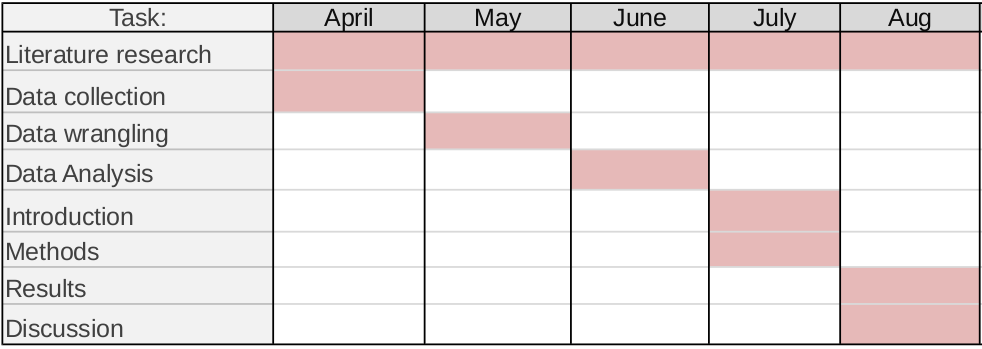
\includegraphics[width=0.4\textwidth]{project.png}
\caption{\label{fig:project.png}Time allocated towards each task to complete the project within 5 months.}
\end{figure}
\section*{Budget}
The budget allocated towards this Master's project is $\pounds 500$. Currently there are no expenses, however future expenses may be towards High Performance Computing time, attending conferences and lab equipment.

\newpage
\thispagestyle{empty}
\section*{Supervisor Statement}
I have seen and approved the proposal and the budget. 
\\
\\Supervisor: Samraat Pawar \\
\\
Signature:  Samraat Pawar\\
\\
Date: 06/04/18

\bibliographystyle{agsm}
\bibliography{refs}

\end{document}

